\documentclass[12pt, a4paper, oneside, openright, titlepage]{book}
\usepackage[utf8]{inputenc}
\raggedbottom
\usepackage{import}


%%%%%%%%%%%%%%%%% Book Formatting Comments:

%%%%%%%%%%%%%%%%%%%%%%%%%%%%%%%%%%%%% for Part

%%%%%%%%%%%%%%%%%%%%%% for chapter

%%%%%%%%%%%%%%%%%%%% for section




%%%%%% PACKAGES %%%%%%%
\usepackage{hyperref}
\hypersetup{
    colorlinks,
    citecolor=black,
    filecolor=black,
    linkcolor=black,
    urlcolor=black
}
\usepackage{amsmath} % Math display options
\usepackage{amssymb} % Math symbols
%\usepackage{amsfonts} % Math fonts
%\usepackage{amsthm}
\usepackage{mathtools} % General math tools
\usepackage{array} % Allows you to write arrays
\usepackage{empheq} % For boxing equations
% \usepackage{mathabx}
% \usepackage{mathrsfs}
\usepackage{nameref}
\usepackage{wrapfig}

\usepackage{soul}
\usepackage[normalem]{ulem}

\usepackage{txfonts}
\usepackage{cancel}
\usepackage[toc, page]{appendix}
\usepackage{titletoc,tocloft}
\setlength{\cftchapindent}{1em}
\setlength{\cftsecindent}{2em}
\setlength{\cftsubsecindent}{3em}
%\setlength{\cftsubsubsecindent}{4em}
\usepackage{titlesec}

%\titleformat{\section}
%  {\normalfont\fontsize{25}{15}\bfseries}{\thesection}%{1em}{}
%\titleformat{\section}
%  {\normalfont\fontsize{20}{15}\bfseries}%{\thesubsection}{1em}{}
%\setcounter{secnumdepth}{1}  
  
  

%\newcommand\numberthis{\refstepcounter{equation}\tag{\theequation}} % For equation labelling
\usepackage[framemethod=tikz]{mdframed}

\usepackage{tikz} % For drawing commutative diagrams
\usetikzlibrary{cd}
\usetikzlibrary{calc}
\tikzset{every picture/.style={line width=0.75pt}} %set default line width to 0.75p

\usepackage{datetime}
\usepackage[margin=1.5in]{geometry}
\setlength{\parskip}{1em}
\usepackage{makeidx}         % allows index generation
\usepackage{graphicx}       % standard LaTeX graphics tool
\usepackage{multicol}        % used for the two-column index
\usepackage[bottom]{footmisc}% places footnotes at page bottom

\usepackage{newtxtext}       % 
\usepackage{newtxmath}       % selects Times Roman as basic font
\usepackage{float}
\usepackage{fancyhdr}
\setlength{\headheight}{15pt} 
\pagestyle{fancy}
\lhead[\leftmark]{}
\rhead[]{\leftmark}

%\usepackage{enumitem}

\usepackage{url}
\allowdisplaybreaks

%%%%%% ENVIRONMENTS %%%
\definecolor{purp}{rgb}{0.29, 0, 0.51}
\definecolor{bloo}{rgb}{0, 0.13, 0.80}



%%\newtheoremstyle{note}% hnamei
%{3pt}% hSpace above
%{3pt}% hSpace belowi
%{}% hBody fonti
%{}% hIndent amounti
%{\itshape}% hTheorem head fonti
%{:}% hPunctuation after theorem headi
%{.5em}% hSpace after theorem headi
%{}% hTheorem head spec (can be left empty, meaning ‘normal’)i





% %%%%%%%%%%%%% THEOREM DEFINITIONS

\spnewtheorem{axiom}{Axiom}[chapter]{\bfseries}{\itshape}


\spnewtheorem{construction}{Construction}[chapter]{\bfseries}{\itshape}

\spnewtheorem{props}{Properties}[chapter]{\bfseries}{\itshape}


\renewcommand{\qedsymbol}{$\blacksquare$}


\numberwithin{equation}{section}

\newenvironment{qest}{
    \begin{center}
        \em
    }
    {
    \end{center}
    }

%%%%%% MACROS %%%%%%%%%
%% New Commands
\newcommand{\ip}[1]{\langle#1\rangle} %%% Inner product
\newcommand{\abs}[1]{\lvert#1\rvert} %%% Modulus
\newcommand\diag{\operatorname{diag}} %%% diag matrix
\newcommand\tr{\mbox{tr}\.} %%% trace
\newcommand\C{\mathbb C} %%% Complex numbers
\newcommand\R{\mathbb R} %%% Real numbers
\newcommand\Z{\mathbb Z} %%% Integers
\newcommand\Q{\mathbb Q} %%% Rationals
\newcommand\N{\mathbb N} %%% Naturals
\newcommand\F{\mathbb F} %%% An arbitrary field
\newcommand\ste{\operatorname{St}} %%% Steinberg Representation
\newcommand\GL{\mathbf{GL}} %%% General Linear group
\newcommand\SL{\mathbf{SL}} %%% Special linear group
\newcommand\gl{\mathfrak{gl}} %%% General linear algebra
\newcommand\G{\mathbf{G}} %%% connected reductive group
\newcommand\g{\mathfrak{g}} %%% Lie algebra of G
\newcommand\Hbf{\mathbf{H}} %%% Theta fixed points of G
\newcommand\X{\mathbf{X}} %%% Symmetric space X
\newcommand{\catname}[1]{\normalfont\textbf{#1}}
\newcommand{\Set}{\catname{Set}} %%% Category set
\newcommand{\Grp}{\catname{Grp}} %%% Category group
\newcommand{\Rmod}{\catname{R-Mod}} %%% Category r-modules
\newcommand{\Mon}{\catname{Mon}} %%% Category monoid
\newcommand{\Ring}{\catname{Ring}} %%% Category ring
\newcommand{\Topp}{\catname{Top}} %%% Category Topological spaces
\newcommand{\Vect}{\catname{Vect}_{k}} %%% category vector spaces'
\newcommand\Hom{\mathbf{Hom}} %%% Arrows

\newcommand{\map}[2]{\begin{array}{c} #1 \\ #2 \end{array}}

\newcommand{\Emph}[1]{\textbf{\ul{\emph{#1}}}}




%% Math operators
\DeclareMathOperator{\ran}{Im} %%% image
\DeclareMathOperator{\aut}{Aut} %%% Automorphisms
\DeclareMathOperator{\spn}{span} %%% span
\DeclareMathOperator{\ann}{Ann} %%% annihilator
\DeclareMathOperator{\rank}{rank} %%% Rank
\DeclareMathOperator{\ch}{char} %%% characteristic
\DeclareMathOperator{\ev}{\bf{ev}} %%% evaluation
\DeclareMathOperator{\sgn}{sign} %%% sign
\DeclareMathOperator{\id}{Id} %%% identity
\DeclareMathOperator{\supp}{Supp} %%% support
\DeclareMathOperator{\inn}{Inn} %%% Inner aut
\DeclareMathOperator{\en}{End} %%% Endomorphisms
\DeclareMathOperator{\sym}{Sym} %%% Group of symmetries


%% Diagram Environments
\iffalse
\begin{center}
    \begin{tikzpicture}[baseline= (a).base]
        \node[scale=1] (a) at (0,0){
          \begin{tikzcd}
           
          \end{tikzcd}
        };
    \end{tikzpicture}
\end{center}
\fi




\newdateformat{monthdayyeardate}{%
    \monthname[\THEMONTH]~\THEDAY, \THEYEAR}
%%%%%%%%%%%%%%%%%%%%%%%

%%% Specific Macros %%%


%%%%%% BEGIN %%%%%%%%%%


\begin{document}

%%%%%% TITLE PAGE %%%%%

\begin{titlepage}
    \centering
    \scshape
    \vspace*{\baselineskip}
    \rule{\textwidth}{1.6pt}\vspace*{-\baselineskip}\vspace*{2pt}
    \rule{\textwidth}{0.4pt}
    
    \vspace{0.75\baselineskip}
    
    {\LARGE Differential Equations: A Complete Guide}
    
    \vspace{0.75\baselineskip}
    
    \rule{\textwidth}{0.4pt}\vspace*{-\baselineskip}\vspace{3.2pt}
    \rule{\textwidth}{1.6pt}
    
    \vspace{2\baselineskip}
    Differential Equations \\
    \vspace*{3\baselineskip}
    \monthdayyeardate\today \\
    \vspace*{5.0\baselineskip}
    
    {\scshape\Large Elijah Thompson, \\ Physics and Math Honors\\}
    
    \vspace{1.0\baselineskip}
    \textit{Solo Pursuit of Learning}
    \vfill
    \enlargethispage{1in}
    \begin{figure}[b!]
    \makebox[\textwidth]{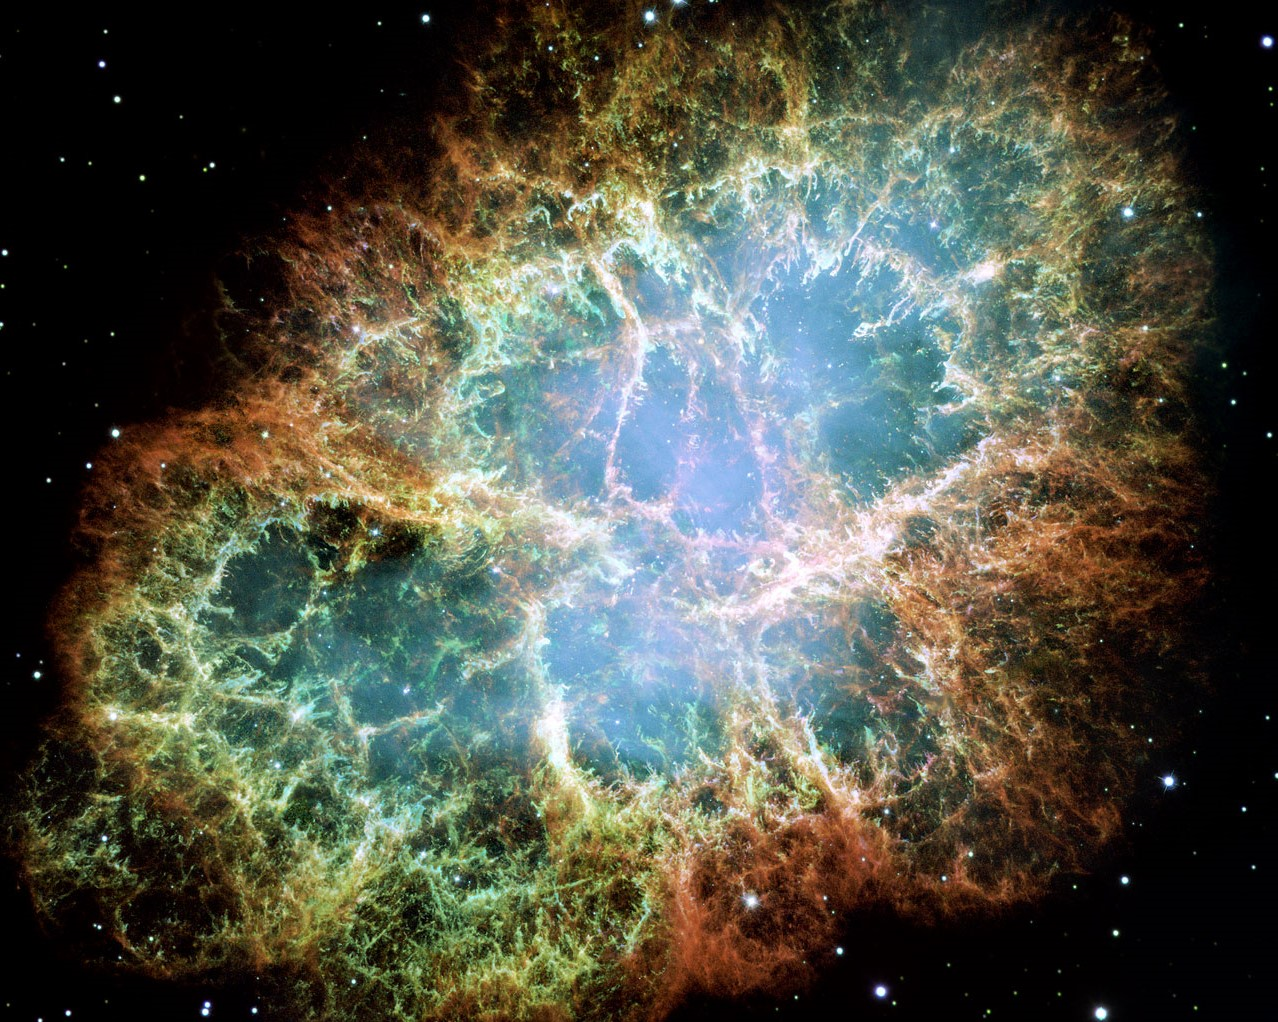
\includegraphics[width=\paperwidth, height =10cm]{../../Crab.jpg}}
    \end{figure}
\end{titlepage}

%%%%%%%%%%%%%%%%%%%%%%%
\tableofcontents








%%%%%%%%%%%%%%%%%%%%%%%%%%%%%%%%%%%%% Part 1. 
\part{Ordinary Differential Equations}




%%%%%%%%%%%%%%%%%%%%%%%%%%%%%%%%%%%%% Part 2.
\part{Partial Differential Equations}



%%%%%%%%%%%%%%%%%%%%%% 2.1
\chapter{Where do PDEs Come From?}

%%%%%%%%%%%%%%%%%%%% 2.1.1
\section{What is a PDE: Notation and Definitions}

\subsection{Partial Derivatives}

Consider a function $u$ of several variables: \begin{equation*}
    u = u(x,y,z)\;\text{ or more generally }\;u = u(x_1,x_2,...,x_n)
\end{equation*}
for $(x,y,z) \in U \subset \R^3$ or $(x_1,x_2,...,x_n) \in U \subset \R^n$. We also write $\mathbf{x} = \vec{x} = (x_1,x_2,...,x_n)$. The $x_1,...,x_n$ are called \Emph{independent variables}

\begin{defn}
    We say that $U \subseteq \R^n$ is a domain if and only if $U$ is connected, $U^{\circ} \neq \emptyset$, and $\partial U$ is smooth.
\end{defn}

\begin{nota}
    Let $u:U\subset \R^n\rightarrow \R$ be a smooth function (e.g. $u \in C^1(U)$). We denote the partial derivatives with \begin{equation*}
        \lim\limits_{h\rightarrow 0}\frac{u(\mathbf{x}+he_i)-u(\mathbf{x})}{h} = \frac{\partial u}{\partial x_i}(\mathbf{x}) = u_{x_i}(\mathbf{x}), \;\;\;i = 1,2,...,n
    \end{equation*}
    where $e_i$ is the $i$th standard basis vector in $\R^n$. For partial derivatives of order $k \in \N$, we write \begin{equation*}
        \frac{\partial^ku}{\partial x_{i_1}...\partial x_{i_k}}(\mathbf{x}) = u_{x_{i_1},...,x_{i_k}}(\mathbf{x}),\;\;i_1,...,i_k \in \{1,...,n\}
    \end{equation*}
    For the collection of all partial derivatives of order $k \in \N$ we write \begin{equation*}
        D^ku := \{u_{x_{i_1},...,x_{i_k}}:i_1,...,i_k \in \{1,...,n\}\} 
    \end{equation*}
\end{nota}

\subsection{Differential Operators}

\begin{defn}
    For $u:U\subset \R^n\rightarrow \R$ smooth, we define the \Emph{gradient} of $u$ to be \begin{equation*}
        \nabla u := (u_{x_1},...,u_{x_n})
    \end{equation*}
    where $\nabla$ is the Nabla differential operator.
\end{defn}

\begin{defn}
    Given a vector $v = (v_1,...,v_n) \in \R^n$ and $u:U\subseteq \R^n\rightarrow \R$ smooth, the directional derivative of $u$ in the direction of $v$ is given by (by application of the chain rule):\begin{equation*}
        D_vu = \nabla u\cdot v = \sum_{i=1}^nu_{x_i}v_i =: \frac{\partial u}{\partial v}
    \end{equation*}
    In particular, $\nabla u\cdot e_i = u_{x_i}$.
\end{defn}

\begin{defn}
    For $V:U\subset \R^n\rightarrow \R^n$ a smooth vector field, we write $V(\mathbf{x}) = (V^1(\mathbf{x}),...,V^n(\mathbf{x}))$, and we have the differential of $V$, or Jacobian, \begin{equation*}
        J_V = DV = \begin{bmatrix} V_{x_1}^1 & \hdots & V_{x_n}^1 \\ \vdots & \ddots & \vdots \\ V_{x_1}^n & \hdots & V_{x_n}^n \end{bmatrix}
    \end{equation*}
    We then define the \Emph{divergence} of $V$ to be \begin{equation*}
        \text{Div}V:= \nabla\cdot V = \text{tr}DV = \sum_{i=1}^nV^i_{x_i} 
    \end{equation*}
\end{defn}

\begin{defn}
    Let $u(\mathbf{x}) = u(x_1,...,x_n)$ be a smooth real-valued function, $\mathbb{x} \in U$. Then $\nabla u:U\subset \R^n\rightarrow \R^n$ and as above we have Hessian matrix for $u$, i.e. the Jacobian of the gradient of $u$: \begin{equation*}
        H_u = D\nabla u = \begin{bmatrix} u_{x_1,x_1} & \hdots & u_{x_1,x_n} \\ \vdots & \ddots & \vdots \\ u_{x_n,x_1} & \hdots & u_{x_n,x_n} \end{bmatrix}
    \end{equation*}
    and we then define the \Emph{laplacian} of $u$ to be the divergence of $\nabla u$: \begin{equation*}
        \Delta u:= \text{tr}D\nabla u = \sum_{i=1}^nu_{x_i,x_i} 
    \end{equation*}
\end{defn}



%%%%%%%%%%%%%%%%%%%% 2.1.2
\section{What is a Partial Differential Equation (PDE)?}

\begin{defn}
    A PDE is an equation which relates an unknown function $u$, its partial derivatives, and its independent variables. 
\end{defn}

A general PDE on a domain $U \subseteq \R^n$ can be written as \begin{equation}
    F(\mathbf{x},u,D^1u,...,D^ku) = F(\mathbf{x},u(\mathbf{x}),D^1u(\mathbf{x}),...,D^ku(\mathbf{x})) = g(\mathbf{x}),\;\;\;\mathbf{x} \in U
\end{equation}
for functions $g(\mathbf{x})$ and $F(\mathbf{x},\theta,\theta^1,...,\theta^k)$, where $(x_1,...,x_n) = \mathbf{x} \in U$, $\theta \in \R$, and $\theta^i = (\theta^i_1,...,\theta^i_{n^i}) \in \R^{n^i}$ and $i = 0,1,...,k$, representing that for a potential function $u:U\subset\R^n\rightarrow \R$, there are $n^i$ partial derivatives of order $i$. $u$ and $D^1u,...,D^ku$ are also called dependent variables.

When we study a PDE often the domain $U$ is not specified yet in the beginning.

\begin{defn}
    The \Emph{order} of a PDE is the highest order of a partial derivative that appears in the equation.
\end{defn}

The most general form of a first order PDE for $2$ independent variables is \begin{equation*}
    F(x,y,u(x,y),u_x(x,y),u_y(x,y)) = f(x,y,u,u_x,u_y) = g(x,y)
\end{equation*}


\subsection{Linear PDEs}


\begin{defn}
    A PDE of the form \begin{equation}
        F(\mathbf{x},u,D^1u,...,D^ku) = g(\mathbf{x})
    \end{equation}
    is called a \Emph{linear} if the function \begin{equation*}
        (\theta,\theta^1,...,\theta^k)\in\R\times \R^n\times...\times \R^{n^k}\mapsto F(\mathbf{x},\theta,\theta^1,...,\theta^k)\in \R
    \end{equation*}
    is multilinear (linear in each $\R$ component).
\end{defn}


A linear PDE of order $2$ in $n$ independent variables can always be written in the form \begin{equation*}
    \sum_{i,j=1}^na_{i,j}(\mathbf{x})u_{x_i,x_j} + \sum_{k=1}^nb_k(\mathbf{x})u_{x_k}+c(\mathbf{x})u = g(\mathbf{x})
\end{equation*}
with coefficients $(a_{i,j}(\mathbf{x}))_{1\leq i,j\leq n},(b_k(\mathbf{x}))_{1\leq k\leq n},c(\mathbf{x})$ that are functions in $\mathbf{x}$.

\begin{eg}[Poisson Equation]
    The Poisson PDE for a function $g:U\subset\R^n\rightarrow \R$ is given by \begin{equation*}
        \Delta u = \sum_{i=1}^nu_{x_i,x_i} = g(\mathbf{x})
    \end{equation*}
    where in the form of the above equation we have $a_{i,j} = \delta_{i,j}$, the Kronecker delta, $b_i = 0$ and $c = 0$.
\end{eg}

\subsection{Nonlinear PDEs}

\begin{defn}
    A PDE of the form $F(\mathbf{x},u,D^1u,...,D^ku) = g(\mathbf{x})$ is called \begin{itemize}
        \item \Emph{semi linear} if we can write \begin{equation*}
                F(\overline{x},\theta,\theta^1,...,\theta^k) = L(\mathbf{x},\theta^k) + G(\mathbf{x},\theta,\theta^1,...,\theta^{k-1})
        \end{equation*}
            and the function $\theta^k \in \R^{n^k}\mapsto L(\mathbf{x},\theta^k)$ is multilinear.
        \item \Emph{quasi linear} if we can write \begin{equation*}
                F(\overline{x},\theta,\theta^1,...,\theta^k) = L(\mathbf{x},\theta,\theta^1,...,\theta^k) + G(\mathbf{x},\theta,\theta^1,...,\theta^{k-1})
        \end{equation*}
            and the function $\theta^k \in \R^{n^k}\mapsto L(\mathbf{x},\theta,\theta^1,...,\theta^k)$ is multilinear.
        \item \Emph{fully nonlinear} if the PDE is not linear, semilinear, or quasilinear.
    \end{itemize}
\end{defn}

The following implications are clear: linear implies semi-linear implies quasi-linear.

Consider a quasi linear PDE $F(\mathbf{x},u,D^1u) = g(\mathbf{x})$. Hence, $F$ has the form \begin{equation*}
    F(\mathbf{x},\theta,\theta^1) = \sum_{i=1}^na_i(\mathbf{x},\theta)\theta^1 + G(\mathbf{x},\theta)
\end{equation*}
The coefficients $(a_i)_{1\leq i \leq n}$ are functions in $\mathbf{x}$ and $\theta$. The PDE takes the form \begin{equation*}
    \sum_{i=1}^na_i(\mathbf{x},u)u_{x_i}+G(\mathbf{x},u) = g(\mathbf{x})
\end{equation*}
\begin{eg}[Inviscid (or Non-viscous) Burger's Equations]
    The PDE \begin{equation*}
        u_t+(u^2)_x = 0 \implies u_t+2uu_x = 0
    \end{equation*}
    is a quasi-linear PDE of order $1$ in $2$ independent variables: $t = x_1$ and $x = x_2$. Here we have $a_1(\mathbf{x},u) = 1, a_2(\mathbf{x},u) = u$ and $G=g \equiv = 0$.
\end{eg}

Consider a PDE of order $2$ $F(\mathbf{x},u,D^1u,D^2u)=g(\mathbf{x})$. If the PDE is quasi-linear, it can be written in the general form \begin{equation*}
    \sum_{i,j=1}^na_{i,j}(\mathbf{x},u,D^1u)u_{x_i,x_j}+G(\mathbf{x},u,D^1u)= g(\mathbf{x})
\end{equation*}
$(a_{i,j})_{1\leq i,j\leq n}, G$ are functions in $\mathbf{x},\theta$, and $\theta^1$.

\subsection{Solutions}

\begin{defn}
    Consider a PDE of order $k$: \begin{equation*}
        F(\mathbf{x},u,D^1u,...,D^ku) = g(\mathbf{x})
    \end{equation*}
    A classical solution of the PDE on a domain $\Omega \subset\R^n$ where $n$ is the number of independent variables, is a sufficiently smooth function $u(\mathbf{x})$ that satisfies it. By sufficiently smooth, we mean in this case that $u \in C^k(\Omega)$.
\end{defn}



\begin{eg}
    The function $u(x,t) = \frac{x}{t}$ solves \begin{equation*}
        u_t + uu_x = 0
    \end{equation*}
    on $\R\times (0,\infty)\subset \R^2$, the upper half plane.
\end{eg}

\subsection{Homogeneous/Inhomogeneous Linear PDEs}

\begin{defn}
    Consider a linear PDE of order $k$: $L(\mathbf{x},u,D^1u,...,D^ku) = \mathcal{L}[u] = g(\mathbf{x})$. If $g(\mathbf{x}) \equiv 0$, the PDE is called \Emph{homogeneous}. Otherwise, the PDE is called \Emph{inhomogeneous}.
\end{defn}

\begin{thm}[Superposition Principle]
    If $u$ and $v$ are solutions to the homogeneous linear PDE $L(\overline{x},u,D^1u,...,D^ku) = 0$ on a domain $\Omega\subset \R^n$, then for all $\alpha,\beta \in \R$, $\alpha u + \beta v$ is a solution to the same homogeneous linear PDE on the domain $\Omega$.
\end{thm}

\begin{thm}[Particular Solution]
    If $u$ solves the homogenous linear PDE $\mathcal{L}[u] = 0$ and $w$ solves the inhomogeneous linear PDE $L[w] = g(\mathbf{x})$, then $u+w$ solves the same inhomogeneous linear PDE.
\end{thm}

It follows that $\mathcal{L}$, defined by $\mathcal{L}[u] = L(\mathbf{x},u,D^1u,...,D^ku)$ is a linear differential operator. Hence, it makes sense to specify appropraite function vector spaces $V$ and $W$ such that $u \in V$ and $\mathcal{L}u \in W$. For instance: For a PDE of order $2$, we can choose $V = C^2(\Omega)$ and $W= C^0(\Omega)$. In particular, for a linear PDE of order one for independent variables $x$ and $y$, we could set $V = C^1(\R^2)$ and $W = C^0(\R^2)$.


%%%%%%%%%%%%%%%%%%%%%% - Appendices
\begin{appendices}


\end{appendices}


\end{document}


%%%%%% END %%%%%%%%%%%%%
